\documentclass[thesis.tex]{subfile}

\chapter{Implementation}
\label{ch:implementation}

We give an overview of the existing spatial tiling transformation in Devito (Section~\ref{sec:spatial-tiling}), then discuss our implementation of time-tiling in detail (Section~\ref{sec:time-tiling}).
The latter extends the former, while depending crucially on an initial skewing transformation.
We examine the safeguards necessary to prevent errors caused by improper skewing.
Finally, we consider the implications on sparse loops, one of Devito's raisons d'\^etre.

\section{Spatial tiling in Devito}
\label{sec:spatial-tiling}

Under the existing tiling transformation, tiling is performed over every dimension but the innermost, which benefits from vectorisation.
In the generated stencils, skewing is not required, as dependencies do not cross tile boundaries, instead referencing values computed in the previous time iteration.

\subsection{Remainder loops}
When discussing loop tiling in Section~\ref{sec:bg-loop-tiling}, we constrained our tiles with \texttt{min} constraints.
To deal with the case when the tile size does not divide the extent of the iteration space, Devito instead implements \emph{remainder loops}, which Figures~\ref{fig:tiled-remainder-space} and~\ref{lst:remainder} illustrate.

\begin{figure}[!ht]
	\centering
	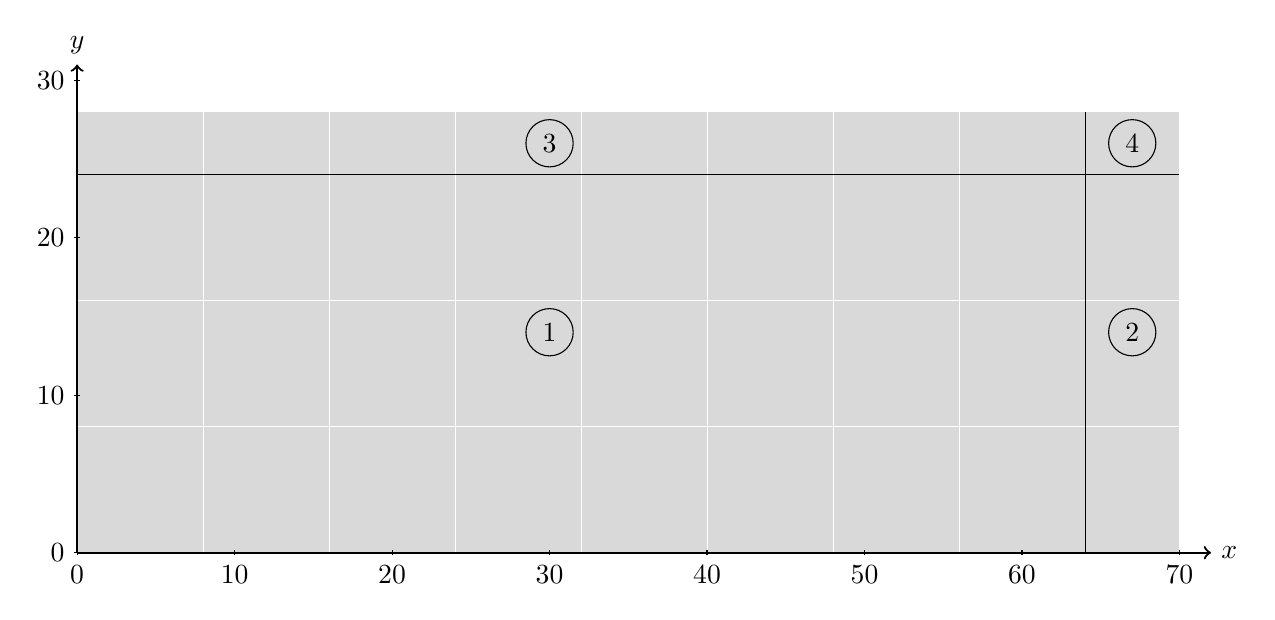
\begin{tikzpicture}
	\fill[gray!30!white] (0,0) rectangle (14,5.6);
	\draw[step=1.6cm,white,very thin] (0,0) grid (14,5.6);

	\draw[thick,->] (0,0) -- (14.4,0) node[right]{$x$};
	\draw[thick,->] (0,0) -- (0,6.2) node[above]{$y$};

	\foreach \x in {0,10,20,30,40,50,60,70}
		\draw (\x*0.2 cm,1pt) -- (\x*0.2 cm,-1pt) node[anchor=north] {$\x$};
	\foreach \y in {0,10,20,30}
		\draw (1pt,\y*0.2 cm) -- (-1pt,\y*0.2 cm) node[anchor=east] {$\y$};

	\draw[xstep=12.8,ystep=4.8,black,very thin] (0,0) grid (14,5.6);
	\draw (6,2.8) circle [radius=0.3] node {$1$};
	\draw (13.4,2.8) circle [radius=0.3] node {$2$};
	\draw (6,5.2) circle [radius=0.3] node {$3$};
	\draw (13.4,5.2) circle [radius=0.3] node {$4$};
	\end{tikzpicture}
	\caption{Tiles over an iteration space. Note that the tile size need not be the same in each dimension, or divide the extent of the iteration cleanly.}
	\label{fig:tiled-remainder-space}
\end{figure}

\begin{figure}[!ht]
\begin{lstlisting}
for (int x_blk = x_s; x_blk < x_e - (x_e-x_s)%x_bs; x_blk += x_bs)
  for (int y_blk = y_s; y_blk < y_e - (y_e-y_s)%y_bs; y_blk += y_bs)
    for (int x = x_blk; x < x_blk + x_bs; x++)
      for (int y = y_blk; y < y_blk + y_bs; y++)
        A[x][y] = B[x][y] + B[x][y+1];  // Nest 1

for (int x = x_e - (x_e-x_s)%x_bs; x < x_e; x++)
  for (int y_blk = y_s; y_blk < y_e - (y_e-y_s)%y_bs; y_blk += y_bs)
    A[x][y] = B[x][y] + B[x][y+1];  // Nest 2

for (int x_blk = x_s; x_blk < x_e - (x_e-x_s)%x_bs; x_blk += x_bs)
  for (int y = y_e - (y_e-y_s)%y_bs; y < y_e; y++)
    A[x][y] = B[x][y] + B[x][y+1];  // Nest 3

for (int x = x_e - (x_e-x_s)%x_bs; x < x_e; x++)
  for (int y = y_e - (y_e-y_s)%y_bs; y < y_e; y++)
    A[x][y] = B[x][y] + B[x][y+1];  // Nest 4
\end{lstlisting}
	\caption{Replacement of \texttt{min} constraints with remainder loops from Figure~\ref{lst:interchange}. First the main tiles, then the remainder in \texttt{x} then \texttt{y} dimensions, and finally the remainders in both dimensions. Braces removed for concision.}
	\label{lst:remainder}
\end{figure}


\section{Skewing and time-tiling}
\label{sec:time-tiling}

As outlined in Section~\ref{sec:bg-time-tiling}, we implement time-tiling in two stages: skewing in the DSE (Section~\ref{sec:dse}), and tiling in the DLE (Section~\ref{sec:dle}).

\subsection{The Devito symbolic engine (DSE)}
\label{sec:dse}

The Devito symbolic engine is responsible for stencil optimisation and common sub-expression elimination.
At this point the indices and loops have not been generated yet.
Although we are working with loop transformations, we chose to perform skewing here, as skewing is a modification on the canonical indexing scheme.

In our implementation, inner loops are skewed by a factor of time, and the loop bounds skewed by the same factor, negated.
This ensures that all accesses refer to the same data as before the transformation, making it valid.
Note that skewing \emph{does not} change the execution order of the loops.

\subsection{The Devito loop engine (DLE)}
\label{sec:dle}

The DLE performs loop transformations including loop fission and tiling, while also marking loops to be executed in parallel or that denormal numbers should be flushed.
Before it is invoked, the loops are built from the previously-manipulated expressions; clearly it would not be possible to implement tiling before this stage.

We then change the tiling algorithm to use the \texttt{min} scheme, rather than remainder loops.
As we noted in the previous section, this will not change the execution order: we now have skewed tiles on a skewed iteration space (Figure~\ref{fig:skewed-loops-skewed-space}).
We now need to `straighten' the tiles by aligning the loop bounds.

% TODO: vague
\begin{figure}[!ht]
	\centering
	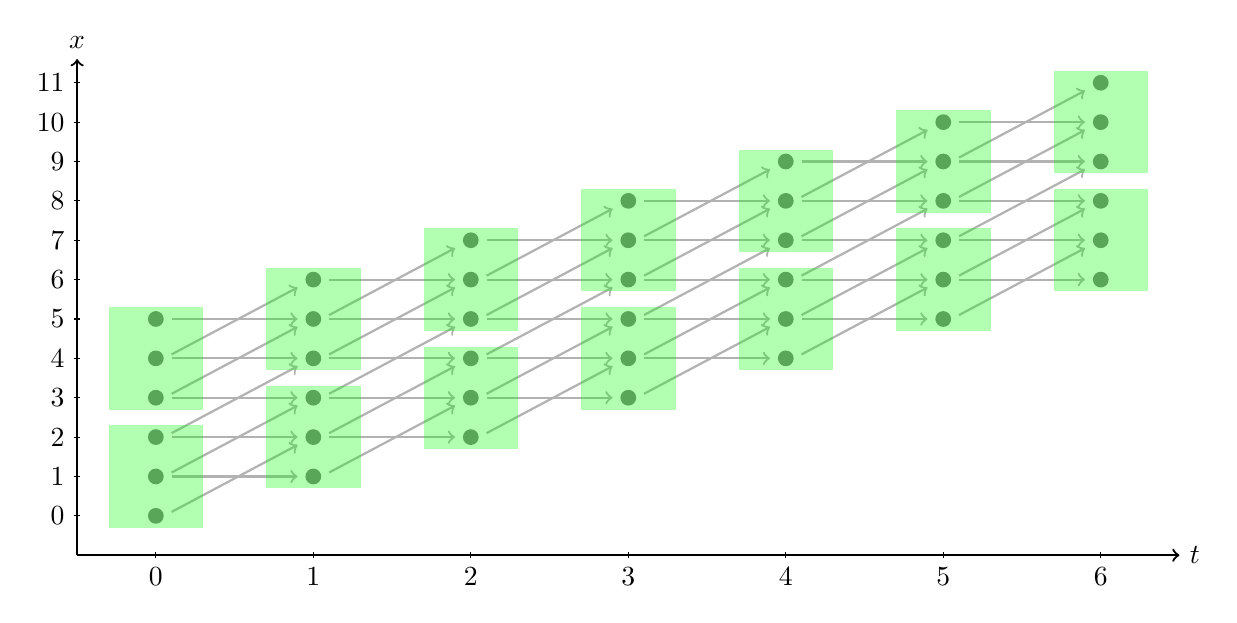
\begin{tikzpicture}
	\draw[thick,->] (-1,-.5) -- (13,-.5) node[right]{$t$};
	\draw[thick,->] (-1,-.5) -- (-1,5.8) node[above]{$x$};
	
	\foreach \t in {0,1,2,3,4,5,6}
	\foreach \x in {0,1,2,3,4,5}
	\fill[gray] (\t*2,\x/2+\t/2) circle (0.1);
	
	\foreach \t in {0,1,2,3,4,5}
	\foreach \x in {1,2,3,4,5}
	\draw[thick,->,gray!60] (\t*2+.2,\x/2+\t/2) -- (\t*2+1.8,\x/2+\t/2);
	
	\foreach \t in {0,1,2,3,4,5}
	\foreach \x in {0,1,2,3,4}
	\draw[thick,->,gray!60] (\t*2+.2,\x/2+\t/2+.05) -- (\t*2+1.8,\x/2+\t/2+.9);
	
	\foreach \t in {0,1,2,3,4,5,6}
	\foreach \x in {0,3}
	\fill[green,opacity=0.3] (\t*2-.6,\x/2+\t/2-.15) rectangle (\t*2+.6,\x/2+\t/2+1.15);
	
	\foreach \t in {0,1,2,3,4,5,6}
	\draw (\t*2,1pt-.5cm) -- (\t*2,-1pt-.5cm) node[anchor=north] {$\t$};
	\foreach \x in {0,1,2,3,4,5,6,7,8,9,10,11}
	\draw (1pt-1cm,\x/2) -- (-1pt-1cm,\x/2) node[anchor=east] {$\x$};
	\end{tikzpicture}
	\caption{Skewed tiles on a skewed iteration space. Dependencies between blocks have not changed, and interchange is not valid.}
	\label{fig:skewed-loops-skewed-space}
\end{figure}

\section{Remaining work}
The implementation work that remains can be divided into several tasks:

\begin{description}
	\item[Straightening of tiles] (end Feb.) This will make the interchange valid, enabling time-tiling. There are a number of concerns:
	\begin{itemize}
		\item The actual straightening, involving some reasoning about loop bounds, use of \texttt{max} -- trivial
		\item Modification to tile the time loop, possibly by incorporating the \texttt{blockshape} parameter -- moderate difficulty due to test cases
		\item Removal of `empty' blocks -- trivial; does not affect correctness but might produce speedup\footnote{CLooG does it, but one has difficulty imagining that there will indeed be a noticeable speedup}
		\item Making this work with time buffering -- some reasoning about skewing factor required
		\item Test cases -- important; partially done
		\item Removal of test cases assuming a remainder loop structure.
		\item Verification that a given skewing factor is valid -- deferred
	\end{itemize}

	\item[Verification of skewing validity] This may be challenging.\footnote{It should be quite easy with knowledge of the data dependence vectors.} For the moment, skewing will work via manual input of skewing factors, hence shifting the responsibility of this onto the user. Clearly, this is not a viable strategy for code acceptance and usage, but it will (minimally) enable our evaluation.

	\item[DSE aggressive mode] Currently, no reason to suppose that this cannot work with \texttt{min}-bounded instead of remainder loops. Need to prove/disprove this, and make it work. Revert to remainder loops if necessary. In particular, we must examine the references made to certain variables.\footnote{Of particular interest are \texttt{blockshape} (the tile size) and dimension extents (e.g.~symbolic extent vs offsets).}

	\item[Sparse loop interpolation] Gather more context and understanding of the problem will be important for reasoning about how this affects time-tiling. Ideally, eventually a proof of what it does/why it does not.

	\item[Detection of when to apply skewing and calculation of the skewing factor] Whether time-tiling is an appropriate optimisation, for a given stencil. Entirely beyond the scope of this work.
\end{description}
